\section{Task Formulation and Dataset}
\label{sec:datasets}
 
Fig. \ref{fig:neuronal-data} briefly illustrates the general pipeline of large-scale neuron reconstruction from EM image volume and various data used in our work.
The huge EM image volume is first over-segmented into a set of 3D segments using an off-the-shelf 3D segmentation approach. Subsequently, human proofreading is performed to obtain complete neurons that usually span several brain regions. The reconstructed neurons are commonly represented by tree structures composed of nodes and edges, either directly traced using annotation software such as CATMAID~\cite{saalfeld2009catmaid} or skeletonized from proofread segment surface using skeletonization algorithms such as TEASAR~\cite{sato2000teasar}. 
For each neuron, we register the over-segmented fragments with the neuron skeleton and obtain the connectivity relations between segments as the ground truth for training and testing.
 
In typical connectomics analysis workflows, human tracers start tracing from an interested neuron branch segment based on the over-segmentation results.
They identify the truncation point by examining its 3D surface mesh. Subsequently, they magnify the questionable area and determine which segment adjacent to the truncation point maintains neuronal continuity with the initial segment of interest, achieved by cross-referencing their 3D meshes and adjacent EM image slices.
For example, to trace the yellow branch in Fig.~\ref{dataset} (in the green box), a human tracer may zoom in to the terminal region, focusing on the lower-left image section. Then, the tracer transits to the adjacent section and sees that the area previously occupied by the yellow segment is now taken over by the blue segment, suggesting a potential connection between them. Typically, tracers proceed to verify their morphological continuity before merging.
   

To relieve the human proofreading workload for huge EM volumes, we propose to predict the connection probability of two segments, $S_a$ and $S_b$, considering their 3D morphology and the EM images from adjacent sections, mimicking the human tracing behavior. We learn the prediction function $f$ from a set of connected segment pairs ($f(S_a, S_b)=1$) that should be merged during proofreading and unconnected pairs ($f(S_a, S_b)=0$). 
 
\subsection{Dataset Construction}
 

\begin{table}[t]
    \caption{Overview of the datasets used in~\cite{matejek2019biologically} and our dataset \textbf{FlyTracing}. N/A denotes that the dataset is not public.
    }
    \centering
    \begin{tabular}{lS[table-format=1.1e2]lS[table-format=1.1e2]}
        \toprule
        \textbf{Dataset} & \textbf{Size ($\mu m^3$)} & \textbf{Method} & \textbf{\# Seg. Pairs} \\
        \midrule
        PNI & $\num{5.0e3}$ & Affinity & N/A \\
        Kasthuri & $\num{5.5e2}$ & Affinity & $\num{1.8e3}$ \\
        SNEMI3D & $\num{5.5e2}$ & Affinity & $\num{\sim e3}$ \\
        \textbf{FlyTracing} & $\num{3.2e6}$ & FFN & $\num{1.6e6}$ \\
        \bottomrule
    \end{tabular}
    \label{dataset-compare}
\end{table}

 \subsubsection{Dataset Overview.}
Available datasets for neural segment connection tasks mainly originated from densely annotated blocks, limited in scale and diversity. 
In contrast, we extract segment connectivity from the crowd-sourced proofreading results throughout an entire fly brain. 
As Table \ref{dataset-compare} shows, our dataset \textbf{FlyTracing} surpasses existing datasets by three orders of magnitude, regarding the volume size and number of connected segment pairs.
The source EM images for FlyTracing are from a complete adult Drosophila brain, imaged at $4\times4 nm$ resolution and sectioned with the thickness of $40 nm$, known as the “full adult fly brain” (FAFB) dataset~\cite{FAFB}. The image sections are first preprocessed through local re-alignment and irregular section substitution, and segmented through a multi-scale FFN segmentation pipeline~\cite{fafb-ffn}, referred to as FAFB-FFN1. The proofread neuron skeletons are supplied by FlyWire~\cite{dorkenwald2022flywire}. 
Despite the availability of affinity-based automatic segmentation from FlyWire, we choose FAFB-FFN1 due to its adherence to over-segmentation consensus, i.e., fewer merging errors than affinity-based segmentation results. 

 \subsubsection{Segment-Neuron Registration.} 
 To generate the ground truth of connectivities of EM segment pairs, we register the FFN segmentation results with the proofread neuron skeletons.
 We design an automatic EM segment-neuron registration method that can be applied to any large-scale connectomics datasets with proofread neuron skeletons and over-segmentation results. 
 With permission from Flywire, we obtain the surface meshes of the proofread neurons and skeletonize them using the skeletor tool~\cite{philipp_schlegel_2022_7308283}. 
 Since we focus on tracing neurites with tree-like structures, we cut off the cell body fibers from the neuron segments.

 
To register the massive over-segmented fragments with a human proofread neuron, given its neuron skeleton $T_{n}$, we associate each skeleton node with its nearest segment.
Since the extracted skeletons and EM image segmentation results inevitably contain errors and noises, a few nodes are occasionally assigned to segments that do not belong to the right neuron. 
To mitigate the assignment errors, we calculate the chamfer distance from the segment skeleton $T_{S}$ to the neuron skeleton $T_{neu}$, subsequently discarding the segments and their corresponding nodes whose $CD(T_{S}, T_{neu})>2\bar{r}$. 
Here, $\bar{r}$ denotes the estimated average radius of the local branch: $\bar{r} = \frac{1}{ |\Omega_S|} \sum_{i\in \Omega_S} r_i$, where $\Omega_S$ is the set of all the neuron skeleton nodes associated to segment $S$. 
%
Once every node is assigned with a corresponding segment, we traverse along the neuron skeleton and identify edges between nodes that are assigned to different segments as bridging edges:
\begin{equation}
    E_{bridge}(T_{neu}) = \{edge(\mathbf{v}_i, \mathbf{v}_j)| S_a \neq S_b\},
\end{equation}
where $\mathbf{v}_i$, $\mathbf{v}_j$ represent two adjacent nodes in $T_{neu}$, and $S_a,S_b$ are their corresponding segments, indicating $S_a$ and $S_b$ should be merged as the same neuron via $edge(\mathbf{v}_i,\mathbf{v}_j)$. 
%
\begin{figure}[t]
    \centering
    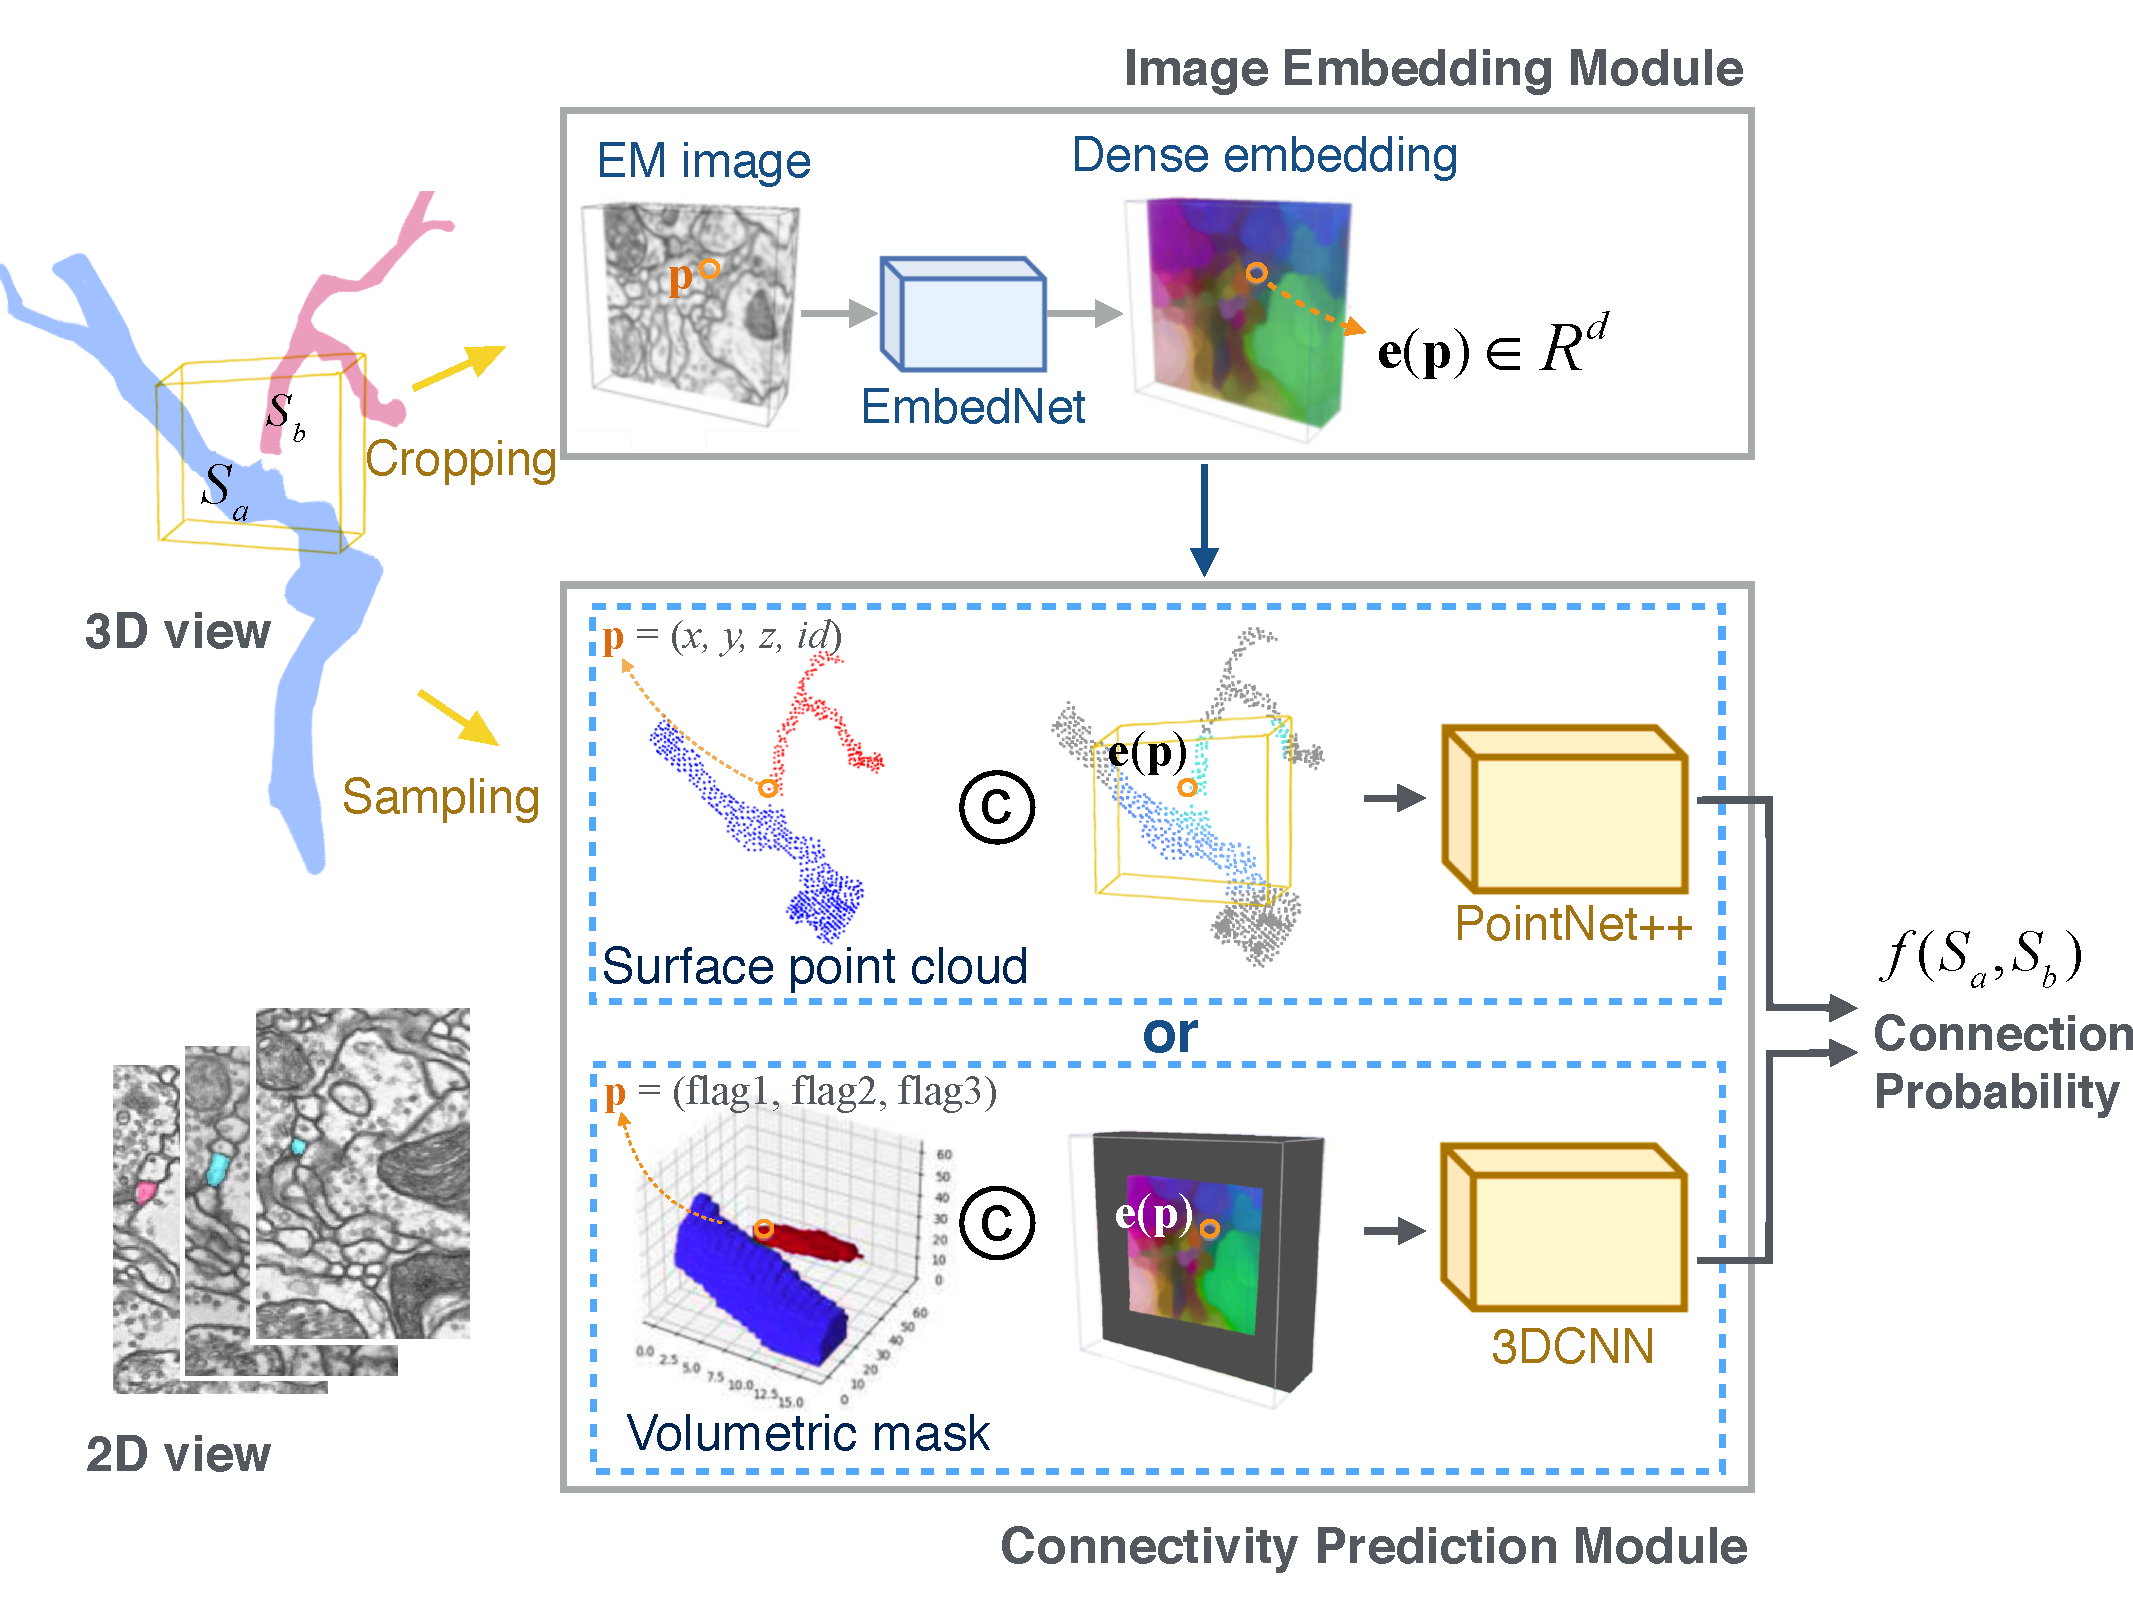
\includegraphics[width=0.48\textwidth]{figs/3Dmodel.pdf}
    \caption{Our connectivity prediction framework fuses local volumetric image features extracted by the EmbedNet with 3D morphology, optionally represented by point cloud or volumetric masks.}% 
    \label{fig:3Dmodel}
\end{figure}

Consequently, we collect the entire bridging edge set from $23,769$ proofread neurons.
The average count of bridging edges per neuron is 810. 
%
For each bridging edge $edge(\mathbf{v}_i, \mathbf{v}_j)$, assuming ${\mathbf{c}}_{i,j}$ is the midpoint of $\mathbf{v}_i$ and $\mathbf{v}_j$, we add random shift to the coordinate of ${\mathbf{c}}_{i,j}$ and obtain ${\hat{\mathbf{c}}}_{i,j}$ as the estimated truncated point. 
The segment pair $(S_a, S_b)$ is annotated as a positive connecting pair ($f(S_a, S_b)=1$).
Any segment $S_c$ that is located in the cube of size $H\times W\times D$ centered at ${\hat{\mathbf{c}}}_{i,j}$ and $S_c \neq S_b$ is labeled with $S_a$ as a negative pair ($f(S_a, S_c)=0$). 


 \subsubsection{Training and Test Block Partition.}
The positive segment pairs across the entire fly brain are partitioned into blocks based on their location in the brain, each spanning a volume size of $26\times 26\times 1\mu m^3$. We select $4,000$ blocks, each of which contains a minimum of $350$ positive segment pairs for training and testing. 
 $1,000$ blocks are selected randomly as the training and validation set for the image embedding network and pairwise connectivity prediction models. The rest $3,000$ blocks are used for testing of connectivity prediction.
 
 